\formdesc{Régime harmonique }   

\underline{Rappel :}

\begin{center}
    \begin{tikzpicture}
        \begin{small} 
            \bXInput{E}
            \bXBloc[10]{H}{$G_a(s)$}{E}
            \bXOutput[10]{y}{H}

            \bXLink[$u(t) = U\cdot sin(wt)$]{E}{H}
            \bXLink[$y(t) = Y \cdot sin(wt+\varphi)$]{H}{y}
        \end{small}
    \end{tikzpicture}
\end{center}

donc : $y = |G_a(jw)| \cdot U\;; \;\varphi = arg(G_a(jw))$

La représentation du régime amorti établi,
la fonction de transfert analogique est évaluée sur l'axe imaginaire.
$s = j\omega$ 

en numérique cela donne : 

$u[k] = U\cdot sin(w\,k\,h)$

$y[k] = Y\cdot sin(w\,k\,h+\varphi)$

donc : $y = |G_n(e^{jwh})| \cdot U\;; \;\varphi = arg(G_n(e^{jwh}))$


La représentation du régime amorti établi,
la fonction de transfert numérique est évaluée sur le cercle unité.

Par conséquent, 

$G_a(e^{jwh}) = G_n(z = e^{jwh})$